%% LaTeX Beamer presentation template (requires beamer package)
%% see http://bitbucket.org/rivanvx/beamer/wiki/Home
%% idea contributed by H. Turgut Uyar
%% template based on a template by Till Tantau
%% this template is still evolving - it might differ in future releases!

\documentclass[10pt]{beamer}

\mode<presentation>
{
\usetheme{Malmoe}

\setbeamercovered{transparent}
}

\usepackage{amssymb}% http://ctan.org/pkg/amssymb
\usepackage{pifont}% http://ctan.org/pkg/pifont
\newcommand{\cmark}{\ding{51}}%
\newcommand{\xmark}{\ding{55}}%


\addtobeamertemplate{navigation symbols}{}{%
\usebeamerfont{footline}%
\usebeamercolor[fg]{footline}%
\hspace{1em}%
\insertframenumber/\inserttotalframenumber
}

\useoutertheme{infolines}
\setbeamertemplate{footline}{} 

\usepackage[brazil]{babel}
\usepackage[utf8]{inputenc}
\usepackage{listings}

% font definitions, try \usepackage{ae} instead of the following
% three lines if you don't like this look
\usepackage{mathptmx}
\usepackage[scaled=.90]{helvet}
\usepackage{courier}
\usepackage{url}


\usepackage[T1]{fontenc}

\title{Reprodução de um elemento do artigo \textit{Accelerating Decoupled
Look-ahead via Weak Dependence Removal: A Metaheuristic Approach}}

%\subtitle{}

% - Use the \inst{?} command only if the authors have different
%   affiliation.
%\author{F.~Author\inst{1} \and S.~Another\inst{2}}
\author{Gustavo Ciotto Pinton}

% - Use the \inst command only if there are several affiliations.
% - Keep it simple, no one is interested in your street address.
\institute
{

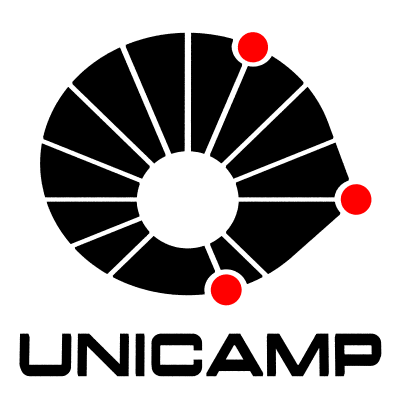
\includegraphics[scale=0.12]{logo} \\
\vspace{16pt}
Universidade Estadual de Campinas - UNICAMP\\
MO601B - Arquitetura de Computadores}

\date{18 de Novembro de 2016}



% If you have a file called "university-logo-filename.xxx", where xxx
% is a graphic format that can be processed by latex or pdflatex,
% resp., then you can add a logo as follows:

% \pgfdeclareimage[height=0.5cm]{university-logo}{university-logo-filename}
% \logo{\pgfuseimage{university-logo}}



% Delete this, if you do not want the table of contents to pop up at
% the beginning of each subsection:
\AtBeginSubsection[]
{
\begin{frame}<beamer>
\frametitle{Outline}
\tableofcontents[currentsection,currentsubsection]
\end{frame}
}

% If you wish to uncover everything in a step-wise fashion, uncomment
% the following command:

%\beamerdefaultoverlayspecification{<+->}

\begin{document}

\begin{frame}

\titlepage
\end{frame}

\begin{frame}
\frametitle{Sumário}
\tableofcontents
\end{frame}

\section{Apresentação do Artigo}
\subsection{Motivação}


\begin{frame}
\frametitle{Motivação}
\begin{itemize}
\item Apesar da proliferação de sistemas \textit{multi-core} e
\textit{multi-threaded}, a performance de aplicações \textit{single-thread}
ainda é um objetivo importante.

\item Aplicações \textit{single-threaded} fazem uso do paralelismo de
instruções.

\item Desafios: como explorar este paralelismo sem muitos custos adicionais

\item Alternativa: \textit{Decoupled look-ahead architecture} 
\end{itemize}

\centering
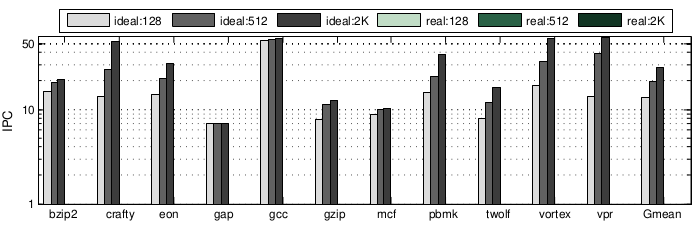
\includegraphics[width=0.9\textwidth]{images/single-ipc}

\end{frame}

\begin{frame}
\frametitle{Motivação}

\begin{itemize}
\item Objetivos da arquitetura \textit{decoupled look-ahed thread}.

\begin{itemize} 
	\item Minimizar os custos de \textit{branch mispredictions} e \textit{cache
	misses}, por exemplo.
	
	\item Explorar oportunidades de paralelismo e o grau de dependência de
	instruções.
  
  	\item Minimizar o consumo energético 
	
\end{itemize} 
\end{itemize}

\vspace{12pt}
\centering
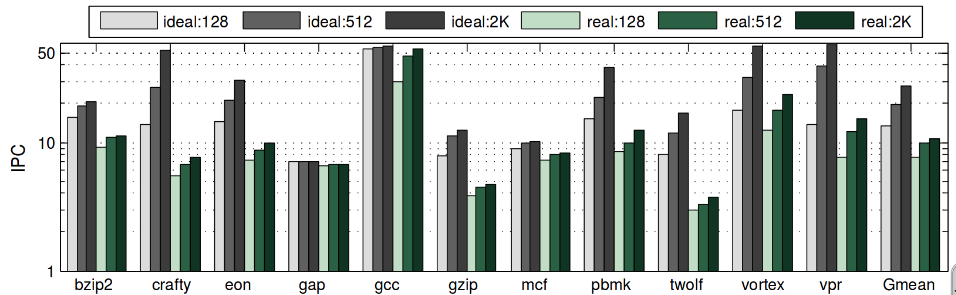
\includegraphics[width=0.9\textwidth]{images/single-ipc-full}

\end{frame}

\begin{frame}
\frametitle{Motivação}

\begin{itemize}
\item Constatou-se que a \textit{thread} auxiliar, isto é, a \textit{look ahead
thread} se tornou o novo limite de velocidade do sistema.

\item A corretude da \textit{look-ahead thread} não é exigida, permitindo várias
otimizações

\begin{itemize} 
	\item Dependências fracas: instruções que contribuem marginalmente para o
	resultado e, portanto, podem ser retiradas.
	
\end{itemize} 

\item O artigo \textit{Accelerating Decoupled
Look-ahead via Weak Dependence Removal: A Metaheuristic Approach} propõe uma
maneira de otimizá-la:
 
\begin{itemize} 
	\item Identificação dos pontos desnecessários que poderiam ser retirados desta
	\textit{thread}. 
	
	\item Como identificá-los automaticamente?
	 
	\item Uso de algoritmos genéticos.
  
  	\item Como caracterizar um gene? 
	
\end{itemize} 
\end{itemize}

\end{frame}

\subsection{Arquitetura Decoupled Look-Ahead}

\begin{frame}
\frametitle{Arquitetura \textit{Decoupled Look-Ahead}}

\begin{itemize}
\item \textit{Parser} que transforma o binário do programa principal em uma
versão reduzida, somente para procurar \textit{misses}.
\item Versão esqueleto roda em \textit{core} separado, anteriormente ao programa
principal.
\item Os resultados de saltos condicionais são transmitidos através
de uma fila para o \textit{core}.
\end{itemize}

\centering
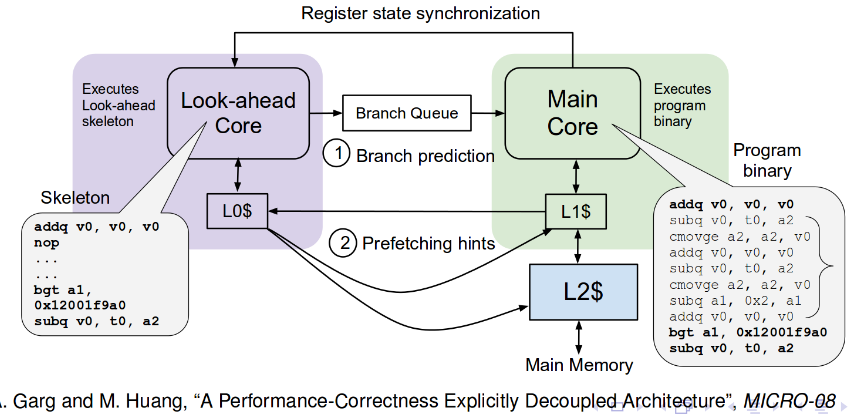
\includegraphics[width=0.9\textwidth]{images/look-ahead}

\end{frame}

\begin{frame}
\frametitle{Arquitetura \textit{Decoupled Look-Ahead}}
\framesubtitle{Dependências fracas}

\begin{itemize}
 \item Instruções que contribuem o mínimo para os propósitos da \textit{lookup
ahead thread}.
\vspace{12pt}
\item Exemplos:
\begin{itemize}
	\item Instruções aritméticas e lógicas que não mudam o resultado de um
	registrador na maior parte do tempo: casos 3 e 5.
	\item Ajustes inúteis em registradores (realizar uma operação em um registrador
	sendo que ele será o alvo de um store em seguida): casos 2 e 4.
	\item \textit{Loads/Stores} inúteis: caso 1.
\end{itemize}
\end{itemize}
\end{frame}

\begin{frame}
\frametitle{Arquitetura \textit{Decoupled Look-Ahead}}
\framesubtitle{Dependências fracas}

\centering
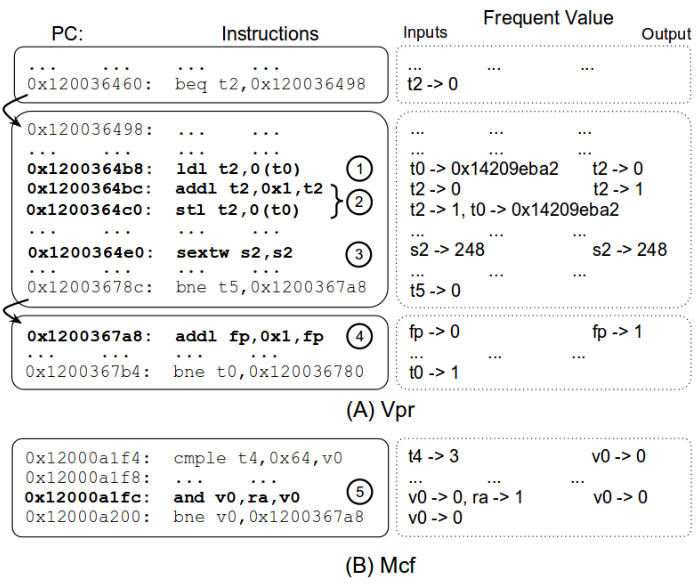
\includegraphics[width=0.7\textwidth]{images/example}

\end{frame}

\begin{frame}
\frametitle{Arquitetura \textit{Decoupled Look-Ahead}}
\framesubtitle{Dependências fracas}

\begin{itemize}
 \item Análise muito difícil caso seja realizada estaticamente: uma
instrução se torna uma dependência fraca de acordo com o contexto do
programa.
\item Nenhuma característica especial em comum que pudesse identificá-las no
momento de geração dos esqueletos. 

\item A identificação de uma instrução errada pode piorar o desempenho do
sistema, dado que novos \textit{misses} podem ser inseridos.
\end{itemize}

\centering
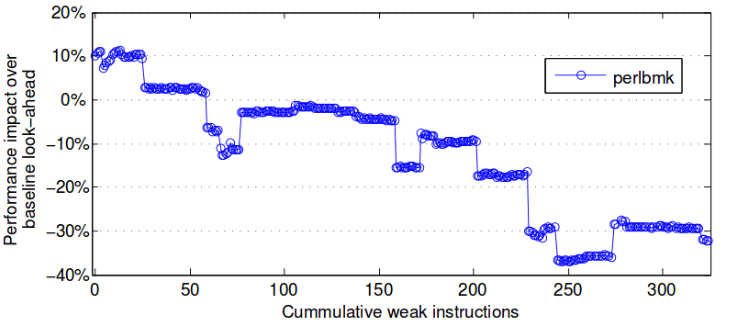
\includegraphics[width=0.7\textwidth]{images/low}

\end{frame}

\begin{frame}
\frametitle{Arquitetura \textit{Decoupled Look-Ahead}}
\framesubtitle{Dependências fracas}

\begin{itemize}
 \item Na figura anterior:
 \begin{itemize}
   \item Após a remoção de 50 dependências fracas, o efeito torna-se negativo.
   \item Em torno de 250 instruções removidas, o pior efeito é encontrado (40\%
   de degradação)
 \end{itemize}
 
 \vspace{12pt}
 
 \item A identificação de um falso positivo é extremamente custoso! 
 
 \vspace{12pt}
 
 \item Dada à natureza dinâmica da evolução das dependências, uma boa maneira
 de encontrar as dependências corretas é o uso de algoritmos genéticos.
\end{itemize}
\end{frame}

\subsection {Implementação Proposta}

\begin{frame}
\frametitle{Implementação Proposta}
\framesubtitle{\textit{Design} básico}

\begin{itemize}
 \item Objetivo: encontrar o esqueleto que maximiza a performance.
 \item Esqueleto = Versão do programa principal após um \textit{filtro}
 \item Algoritmo genético para encontrar o melhor \textit{filtro}:
 \begin{itemize}
   \item Esqueleto é representado por um vetor de \textit{bits}
   \item Mapeamento: instrução fraca \(\rightarrow\) gene, coleção de instr.
   \(\rightarrow\) cromossomo
 \end{itemize}
 
 \vspace{12pt}
 \centering
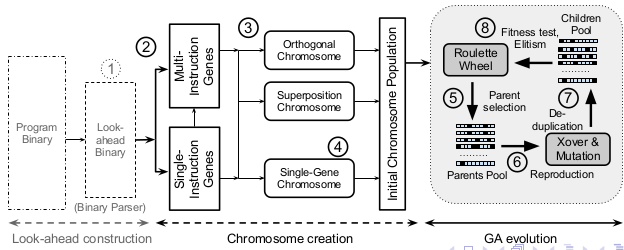
\includegraphics[width=0.8\textwidth]{images/evol}
\end{itemize}
\end{frame}

\begin{frame}
\frametitle{Implementação Proposta}
\framesubtitle{\textit{Design} básico}

\begin{itemize}
  \item Formação da população inicial:
  \begin{itemize}
  	\item \textit{Single-Gene chromosomes}: N cromossomos com apenas um gene
  	\item \textit{Superposition chromosomes}: N - 1 cromossomos gerados a partir
  	da superposição dos genes em ordem crescente de \textit{fitness}
  	\item \textit{Orthogonal chromosomes}: genes obtidos de rotinas distintas
   \end{itemize}
\end{itemize}

 \centering
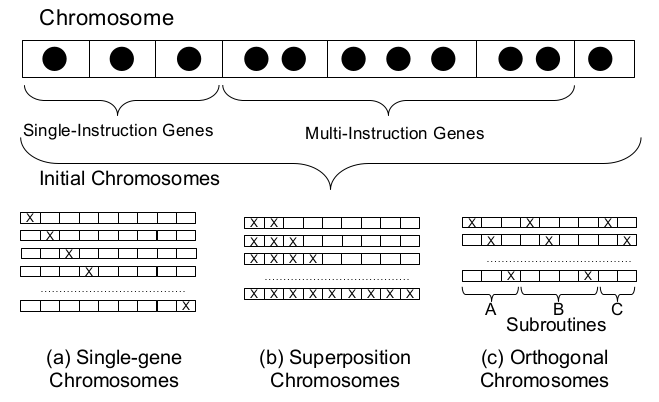
\includegraphics[width=0.7\textwidth]{images/initial}
\end{frame}

\subsection {Resultados}
\begin{frame}
\frametitle{Resultados}
\begin{itemize}
  \item Aumento do desempenho sobre os programas originais: 1.58x
  \item Aumento do desempenho sobre o modelo de \textit{decoupled look-ahed
  thread} original: 1.14x (em média geométrica)
\end{itemize}

\vspace{14pt}

\centering
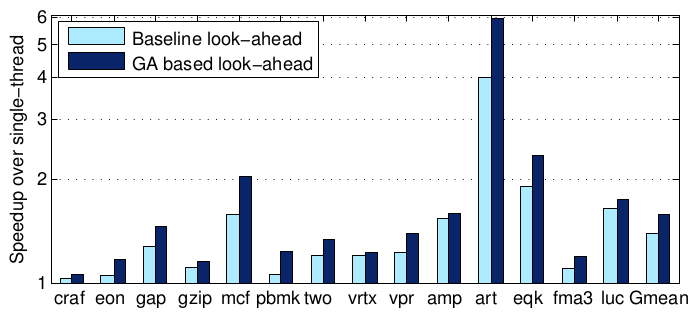
\includegraphics[width=0.7\textwidth]{images/results}
\end{frame}

\section{Reprodução de um elemento do artigo}
\subsection{Elemento escolhido} 
\begin {frame}
\frametitle{Reprodução de um elemento do artigo}
\framesubtitle{Apresentação}
\begin{itemize}
\item Reprodução das curvas \textit{ideal} e \textit{single-thread} da figura 3.
\end{itemize}

\vspace{16pt}
\centering
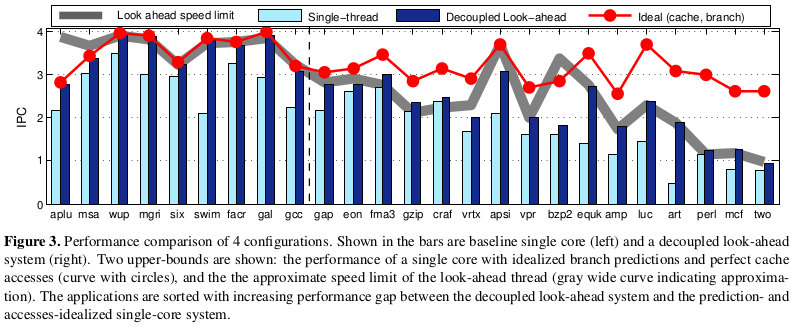
\includegraphics[width=1\textwidth]{images/fig3} 
\end{frame}

\subsection{Configuração}

\begin {frame}
\frametitle{Reprodução de um elemento do artigo}
\framesubtitle{Configuração do \textit{sniper}}
\begin{itemize}
\item Máquina virtual de 64 bits Ubuntu 14.04 LTS.
\item Compilado com o gcc 4.4.
\item Dois tipos de pinballs do \texttt{SPEC CPU2006} foram utilizados: 
\begin{itemize}
  \item 100M instruções de warmup e 30M instruções na região detalhada.
  \item 1B de instruções na região detalhada e sem warmup.
\end{itemize}

\item Integração dos \textit{pinballs} com o \textit{sniper}: 
\begin{itemize}
  \item \textit{Pinballs} de 1B de instruções: apenas acrescentar
  \texttt{--pinballs=<\ldots>}
  \item \textit{Pinballs} de 100M+30M de instruções: diversas tentativas
\end{itemize}
\end{itemize} 
\end{frame}

\begin {frame}
\frametitle{Reprodução de um elemento do artigo}
\framesubtitle{\textit{Pinballs} de 100M+30M}
\begin{itemize}
  \item Opção \texttt{--roi}: o \textit{pinball} é
  executado integralmente em modo \texttt{CACHE\_ONLY}, gerando nenhum arquivo de
  saída e nenhuma estatística. \xmark
  \vspace{12pt}
  \item Implementação de \textit{pintool}: conta as instruções e chama a função
  \texttt{SimRoiStart()} explicitamente (\path{sniper/include/sim_api.h}) \xmark
  \begin{itemize}
    \item \textit{Sniper} não é capaz de executar o binário do pin, uma vez que este
    último foi pré-compilado em uma máquina de 32 bits.
  \end{itemize}
  \vspace{12pt}
  \item Máquina virtual de 32 bits: compilação do \textit{sniper}. \xmark
  \begin{itemize}
    \item \textit{Pinballs} criados em máquinas de 64 bits e não podem rodar em máquinas de 32 bits.
  \end{itemize}
  \vspace{12pt}
  \item \textit{Script} python com a opção \texttt{-s}: script python capaz de
  contar as instruções é disponível no diretório \path{sniper/scripts}. \cmark
  
  \begin{itemize}
    \item \texttt{roi-icount.py}: deve ser chamado com o parâmetro
    0:100000000:30000000
  \end{itemize}

\end{itemize}

\end{frame}

\begin{frame}
\frametitle{Reprodução de um elemento do artigo}
\framesubtitle{Ambiente de testes}

\begin{itemize}
  \item Linhas indicadas por \cmark: corretamente configuradas
  \textit{sniper}.
  \item Linhas indicadas por \xmark: modificações mais profundas no modelo de
  intervalos do \textit{sniper}.
\end{itemize}

\begin{table}[h]
    \centering
	\begin{tabular}{| l | l | l | }
		\hline
		\multicolumn{3}{|c|}{ \textbf{Baseline core}} \\ \hline
		Fetch/Decode/Issue/Commit & 8/4/6/6 & \xmark\\ 
		ROB & 128 & \cmark \\ 
		Functional units & INT 2+1 mul +1 div, FP 2+1 mul +1 div & \xmark\\
		Fetch Q/ Issue Q / Reg. (int,fp) & (32, 32) / (32, 32) / (80, 80) & \xmark\\ 
		LSQ(LQ,SQ) & 64 (32,32) 2 search ports & \xmark\\
		Branch predictor & Gshare – 8K entries, 13 bit history & \cmark \\ 
		Br. mispred. penalty & at least 7 cycles & \cmark \\ 
		L1 data cache (private) & 32KB, 4-way, 64B line, 2 cycles, 2 ports &
		\cmark \\
		L1 inst cache (private) & 64KB, 2-way, 128B, 2 cycles & \cmark \\ 
		L2 cache (shared) & 1MB, 8-way, 128B, 15 cycles & \cmark \\ 
		Memory access latency & 200 cycles & \cmark \\ \hline
		
	\end{tabular}
\end{table}

\end{frame}

\begin{frame}
\frametitle{Reprodução de um elemento do artigo}
\framesubtitle{Arquivos de configuração}

\begin{itemize}
  
  \item \textit{Core} modelado pela microarquitetura \textit{Nehalem} (padrão do
  \textit{sniper})
  \begin{itemize} 
  \item Modelar POWER5 : projeto 4!
  \end{itemize}
  
  \vspace{12pt}
  \item \textit{Caches} ideais:
 
  \begin{itemize} 
  \item \texttt{perf\_model/tlb/penalty = 0}
  \item \texttt{perf\_model/l1\_icache/perfect=true}
  \item \texttt{perf\_model/l1\_dcache/perfect=true}
  \item \texttt{perf\_model/l2\_cache/perfect=true} 
  \end{itemize}

\vspace{12pt}
\item \textit{Branch predictor} ideal:
  \begin{itemize} 
  \item \texttt{perf\_model/branch\_predictor/mispredict\_penalty=0}
  \end{itemize}
\end{itemize}
\end{frame}

\begin{frame}
\frametitle{Reprodução de um elemento do artigo}
\framesubtitle{Implementação do preditor \textit{gshare}}

\begin{itemize}
  
  \item Definição da classe abstrata \texttt{BranchPredictor}, possuindo dois
  métodos virtuais:
  \begin{itemize} 
  \item \texttt{predict()} : retorna um \textit{booleano}
  \item \texttt{update()}: atualiza preditor de acordo com o resultado.
  \end{itemize}
 
 \item Implementação disponível: preditor de dois \textit{bits}
 \texttt{SaturatingPredictor<2>}
 
 \item \texttt{predict()}:
  \begin{itemize} 
  \item Cálculo do índice: \texttt{indice = (pc XOR global\_history) \& 0x1FFF}
  \item Retornar \texttt{preditores[indice].predict()}
  \end{itemize}
  
  \item \texttt{update()}:
  \begin{itemize} 
  \item Cálculo do índice, conforme acima.
  \item Atualização do registro global:\\ \texttt{global\_history =
  (global\_history << 1) | branch\_outcome}
  \item Atualizar preditor: \texttt{preditores[indice].update(branch\_outcome)}
  \end{itemize}
 
 \item Integração com o \textit{sniper}: através do arquivo
 \texttt{branch\_predictor.cc}.
 

\end{itemize}
\end{frame}

\subsection{Resultados}
\begin{frame}
\frametitle{Reprodução de um elemento do artigo}
\framesubtitle{Resultados}

\begin{itemize}
  \item Uso dos \textit{benchmarks} do \texttt{SPEC CPU2006}, contrariamente ao
  artigo.
  \vspace{10pt}
  \item Apesar de todo trabalho para configurar os \textit{pinballs} de
  100M+30M, eles não foram utilizados
  \begin{itemize}
    \item Resultados muito distantes daqueles encontrados para os de 1B e para
    os do artigo.
  \end{itemize}
  \vspace{10pt}
  \item Duas configurações utilizadas:
  \begin{itemize}
    \item Microarquitetura \textit{Intel Gainestown} para testes
    \item Configuração do artigo
  \end{itemize}
  \vspace{10pt}
  \item \textit{Pinballs} de 1B: média de 30 minutos para cada entrada
  \begin{itemize}
    \item Execução em 4 \textit{cores}
  \end{itemize}
\end{itemize}

\end{frame}

\begin{frame}
\frametitle{Reprodução de um elemento do artigo}
\framesubtitle{Resultados - \textit{Gainestown}}

\centering
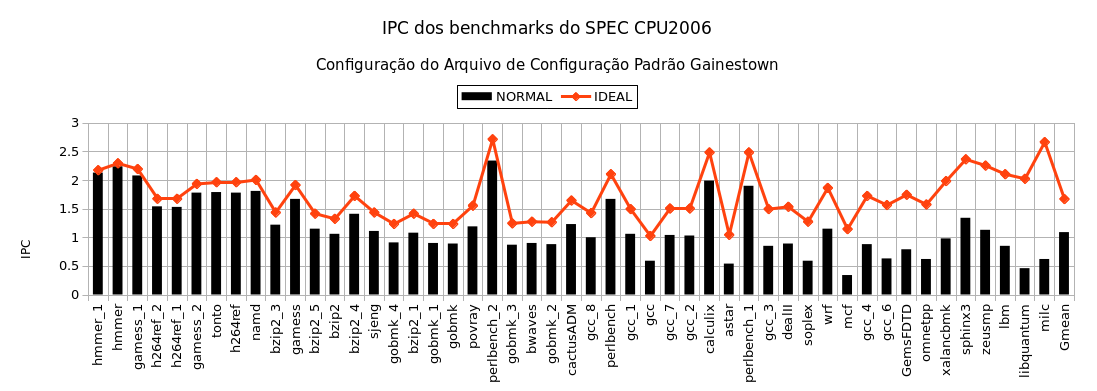
\includegraphics[width=\textwidth]{images/gainestown}

\end{frame}


\begin{frame}
\frametitle{Reprodução de um elemento do artigo}
\framesubtitle{Resultados - \textit{Artigo}}

\centering
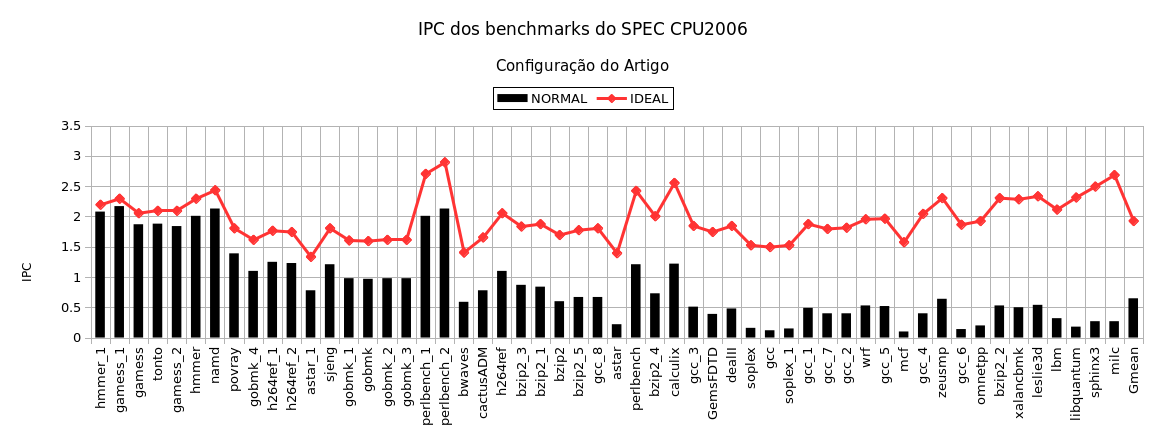
\includegraphics[width=\textwidth]{images/article}

\end{frame}

\subsection{Conclusão}
\begin{frame}
\frametitle{Reprodução de um elemento do artigo}
\framesubtitle{Conclusão}


\begin{itemize}
\item Desempenhos ideais: IPCs muito parecidos entre si.
\begin{itemize}
    \item Artigo: 1.93 (\textit{Gmean}).
    \item \textit{Gainestown}: 1.68 (\textit{Gmean}).  
 \end{itemize}
 \vspace{10pt}
\item As medidas de IPC para os casos normais variam mais
entre si: 
\begin{itemize}
    \item Artigo: 0.65 (\textit{Gmean}).
    \item \textit{Gainestown}: 1.09 (\textit{Gmean}).  
    \item Variação de 1.68x.
 \end{itemize}
\vspace{10pt}
\item Em relação aos resultados encontrados no artigo:
\begin{itemize}
    \item IPCs maiores que os encontrados nos experimentos encontrados neste
    relatório.
    \item \textit{Gainestown}: 1.09 (\textit{Gmean}).  
    \item Autores utilizaram os programas completos! 
 \end{itemize}
 \vspace{10pt}
 \item No nosso caso, uma entrada completa levaria \(\approx\) 500 horas!
\end{itemize}
\end{frame}

\section{Referências}
\begin{frame}
\frametitle{Referências}

\begin{itemize}
  \item Carison, T. E. (2012). Interval simulation.
  \url{http://snipersim.org/w/Interval_ Simulation}. 
\item Carison, T. E. and Heirman, W. (2013). The Sniper User Manual.
\item Parihar, R. and Huang, M. C. (2014). Accelerating decoupled look-ahead via
weak dependence removal: A metaheuristic approach. International Symposium on High Performance Computer Architecture.
\end{itemize}

\end{frame}

\end{document}
